\documentclass[../main.tex]{subfiles}
\begin{document}

Throughout this section, $E$ will denote $\bR^n$ equipped with the standard inner product, our fixed \textit{euclidean space}.

\subsection{Affine reflections}

This subsection roughly follows \cite{Berger2009}. When considering reflections in $E$, we don't want to just consider those lying in $O(E)$, we are also interested in reflections across some hyperplane not lying throught the origin. To tackle this we first define some standard preliminaries:

\begin{definition}
    A \textbf{reflection} in $E$ is a linear transformation $s\in O(E)$ (the orthogonal group of inner product preserving linear maps) with eigenvalues $\{-1,1\}$ with corresponding dimensions of eigenspaces:\[
        \dim{E_1} = n-1 \qquad \dim{E_{-1}} = 1
    \]
    for linear maps in $O(E)$ this is equivalent to fixing some hyperplane (codimension $1$ subspace) and having determinant $-1$.
\end{definition}

\begin{definition}
    The \textbf{group of general affine transformations} of $E$ is semidirect product of $GL(E)$ acting on $E$\[
    GA(E) := E \rtimes GL(E)
    \] where $E$ acts on itself by translation. $(v,T)\in GA(E)$ acts on $e\in E$ as $(v,T)\cdot e = v + T(e)$.
\end{definition}

\begin{proposition}
    This is actually an action. Furthermore, the action is transitive.
    \begin{proof}
        Take $(v,T), (u,S)\in GA(E)$ and $e\in E$. Showing this is an action is a direct calculation: \[
        (v,T) \cdot \pr{(u,S) \cdot e} = (v,T)\cdot \pr{u + S(e)} = v + T(u) + TS(e) = (v+T(u),TS)\cdot e = \pr{(v,T)(u,S)}\cdot e\]
        from the definition of the semidirect product. Suppose $(v,T)$ and $(u,S)$ act the same on $E$: as both $T$ and $S$ are linear the two affine transformations send $0$ to $v$ and $u$ respective, thus we have $v=u$; subtracting these equal translations and having equality means the two linear transformations must also be equal.
    \end{proof}
\end{proposition}

We can now consider appropriate affine versions of linear groups, the most important for us will be the \textbf{affine orthogonal group} $AO(E)$, which can be equivalently viewed as the subgroup of $GA(E)$ preserving the inner product or as $E\rtimes O(E)$. We need stricter criteria than just the linear component of our affine transformation be a reflection to suitably capture the notion of a reflection across an affine hyperplane.

\begin{proposition}
    For a unit normal vector $\alpha$ and some $k\in \bR$, reflection across the affine hyperplane $(E,\alpha) = k$ corresponds to the affine transformation $(2k\alpha,s_\alpha)$, where $s_\alpha$ is the reflection along $\alpha$.\begin{proof}
        Call the affine hyperplane $H$ and choose a $v\in E$. The vector orthogonal to $H$ that goes to $v$ has length $k-(v,\alpha)$ so reflecting across $H$ send $v$ to $v+2(k-(v,\alpha))\alpha = 2k\alpha + (v-2(v,\alpha)\alpha) = (2k\alpha, s_\alpha)\cdot v$.
    \end{proof}
\end{proposition}

We call such affine transformations, \textbf{affine reflections}.

\begin{lemma}
    For all affine hyperplanes $H$ and affine reflections $r$, the set $rH$ is also an affine hyperplane.
    \begin{proof}
        Let $H$ be $\{v\in V \mid (v,\alpha)=k\}$ for some $\alpha\in E, k\in\bR$. As $r$ is bijective the set $rH$ is equal to $\{w\in V \mid (r^{-1}w,\alpha) = k\}$, by writing $r=(u,T)\in GA(E)$ this can be rewritten as $\{w\in V\mid (w,T^*(\alpha))=k-(u,\alpha)\}$, an affine hyperplane.
    \end{proof}
\end{lemma}

\begin{lemma}
    An affine transformations $r=(u,T)$ that fixes some affine hyperplane and is an involution must be an affine reflection.
    \begin{proof}
        As $r^2=\text{id}$, on $0$ we have $r^2(0)=u+T(u)=0$. So as $r^2=u+T(u)+A^2$ this means $A$ is also an involution so we can use the primary decomposition $E=E_1\oplus E_{-1}$ into the eigenspaces of $A$. Call the hyperplane $r$ fixes $H$, then for any $h=v_1+v_{-1}\in H$ (where $v_1,v_{-1}\in V_1,V_{-1}$ respectively) we have $r(v_1+v_{-1}) = u + T(v_1+v_{-1}) = u + v_1 - v_{-1} = v_1 + v_{-1}$ therefore $2v_{-1}=u$ so $\dim E_{-1}=1$ and $T$ is the reflection along $V_{-1}=\abr{v_{-1}}$, thus $r=\pr{2v_{-1},s_{v_{-1}}}$.
    \end{proof}
\end{lemma}

\begin{proposition}
    For all affine reflections $r,s$ with $s$ reflecting across the affine hyperplane $H$, the affine transformation $rsr^{-1}$ is an affine reflection across $rH$.
    \begin{proof}
        First, notice $\pr{rsr^{-1}}^2 = \text{id}$ as both $r$ and $s$ are involutions. Also, $rsr^{-1}(rH) = rH$ as $s$ fixes $H$.
    \end{proof}
\end{proposition}

From now on, we will use the umbrella term \textit{reflection} to refer to both linear and affine reflecitons.

\subsection{Reflection groups}

The plan is to show all finitely generated reflection groups are in fact Coxeter groups, which admit a nice geometric classification. This follows \cite{Humphreys1990}

We are interested in groups generated by reflections in $E$, so throughout the next two sections fix a group $W\leq GA(E)$ which can be generated by reflections.

Consider the set $\cH$ of all hyperplanes such that an element $w\in W$ is the reflection across. If we make a poor choice of our reflections generating $W$ we may end up with $\cH$ dense in $E$.

\begin{example}
    Consider the following set of hyperplanes in $\bR^2$, by previous lemma $\cH$ is closed under the induced action from $W$ so any such pentagon will generate a smaller pentagon, inverted in its center, this infinite descent makes $\cH$ dense in $\bR^2$.
\end{example}

To remedy this we will restrict the reflection groups we consider by rquiring for any compact subset $B\subset E$, the intersection $\cH\cap B$ be finite.

\begin{definition}
    The connected components of $E\setminus \cH$ are called the \textbf{chambers} of $W$ in $E$.
\end{definition}

\begin{proposition}
    The number of hyperplanes touching any single chamber is finite.
\end{proposition}

We now want to choose a chamber $C_0$, and consider the set of hyperplanes $\{H_1,\ldots,H_k\}\subseteq \cH$ bounding $C$. We will call the corresponding reflections across these hyperplanes $\{s_1,\ldots,s_k\}$ \textbf{simple reflections}.

\begin{theorem}
    The set of simple reflections $\{s_1,\ldots, s_k\}$ generates $W$.
    \begin{proof}
        Let $W'$ be the subgorup of $W$ generated by the simple reflections. Let $s$ be one of the reflections generating $W$, and call the hyperplane it reflects across $H$. If $W'$ acts transitively on the set of chambers then there will exists some $w\in W'$ such that $wH_i=H$ for some simple reflection $s_i$ as $H$ will must bound a chamber. Thus, by an earlier lemma, $ws_iw^{-1} = s$ so $s\in W'$ and $W=W'$.
        Now we just have to show the action of $W'$ is transitive on chambers. Suppose it isn't, i.e. there is some chamber $C$ such that no $w\in W'$ satisfies $wC=C_0$. Let $C'$ be the closest chamber to $C_0$ in the $W'$ orbit of $C$, as $C'\neq C_0$ there must be some simple hyperplane (the boundary of $C_0$) between them, reflecting across this must strictly decrease the distance between the two chambers contradicting the minimality of $C'$. Thus $W'$ acts transitively on the set of chambers.
    \end{proof}
\end{theorem}

As a direct corollary of this proof we now know $W$ acts transitively on the set of chambers. Before discussing this further we should examine the relations that these simple reflections satisfy.

For any two simple reflections $s_i,s_j$ the subgroup $\abr{s_i,s_j}$ will be dihedral, as seen in the previous section, (note that this will be the infinite dihedral group iff the hypeplanes being reflected along are parallel), call the order of this dihedral group $2m_{ij}$. The product $s_i s_j$ will have order $m_{ij}$ in $W$ and so $W$ satisfies the set of relations $(s_is_j)^{m_{ij}}=\text{id}$ for all $i,j$, taking $m_{ii}=1$. A group \textit{presented} by these relations is called \textbf{Coxeter}.

\begin{definition}
    A \textbf{Coxeter system} is a pair $(W,S)$ where $S=\{s_i\}_{i\in I}$ is a generating set for $W$ which admits the presentation:\[
        W = \abr{S \mid (s_is_j)^{m_{ij}} \text{ for all } i,j\in I}
    \]
    where each $m_{ij}\in \bN\cup\{\infty\}$.
\end{definition}

To each Coxeter system we can assign a \textbf{Coxeter diagram}: an undirected graph created by the following rules:\begin{itemize}
    \item Draw a node $i$ for each $s_i\in S$;
    \item For each relation $(s_i s_j)^{m_{ij}}$ with $m_{ij}>2$ draw an edge between $i$ and $j$ and label it with $m_{ij}$.
\end{itemize}

This process can be reversed to obtain a Coxeter system from any Coxeter diagram. This correspondence will associate the graph:
\begin{figure}[!h]
\centering
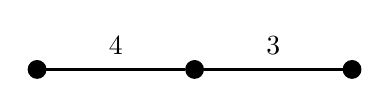
\begin{tikzpicture}
    \begin{scope}[every node/.style={circle, fill=black, draw, thick, minimum size = 6pt, inner sep=0pt}]
        \node (1) at (0,0) {};
        \node (2) at (2,0) {};
        \node (3) at (4,0) {};
    \end{scope}

    \begin{scope}[every edge/.style={draw,very thick}]
        \path [-] (1) edge (2);
        \path [-] (2) edge (3);
        \node at (1,0.3) {$4$};
        \node at (3,0.3) {$3$};
    \end{scope}
\end{tikzpicture}
\end{figure}

to the group presentation: \[
\abr{s_1,s_2,s_3 \ \middle| \ s_1^2 = s_2^2 = s_3^2 = e, \ (s_1s_2)^4 = (s_2s_3)^3 = (s_1s_3)^2 = e}
\]

In the future, for the sake of readability, the $3$ labels will often be excluded.

The classification of finite reflection groups goes by prooving all reflection groups are infact Coxeter groups and then classifying all the finite Coxeter groups.

\subsection{Coxeter presentation}

We have shown the action of $W$ on the set of chambers is transitive, but we need a stronger notion to prove these groups are Coxeter.

\begin{definition}
    Let $G$ be a group acting on a set $X$, the action is called \textbf{simply transitive} if for all $x,y\in G$ there exists a unique $g\in G$ such that $g\cdot x = y$.
\end{definition}

By fixing a base point $x\in X$ there is clear a 1-to-1 correspondence between $X$ and $G$: associate $e\leftrightarrow x$ and for all $g\in G$, $g\leftrightarrow g\cdot x$.

\begin{proposition}
    An action is simply transitive iff it is transitive and free.
    \begin{proof}
        An action is transitive if for all $x,y\in X$ there exists some $g\in G$ such that $g\cdot x = y$, and free if there exists at most one such $g$; therefore these statements are equivalent.
    \end{proof}
\end{proposition}

If we know the action is trasntive a priori we only need to check the free condition on a single element. So showing our action is simply transitive ammounts to showing for all $w\in W$ such that $wC_0 = C_0$ we have $w=\text{id}$.

We will go about prooving this by finding a geometric interpretation of the length of a word $w\in W$ in terms of simple reflections.

\begin{definition}
    For $w\in W$ define the \textbf{length} of $w$, $l(w)$ to be the minimal positive integer $r$ such that $w=s_1\cdots s_r$, a length $r$ product of simple reflections.
\end{definition}

And the contrasting way to compute the length: for any $w\in W$ consider the set of hyperplanes $H$ such that $C_0$ and $wC_0$ lie on different sides of $H$. Call this $\cL(w)$ and let $n(w) = |\cL(w)|$.

\begin{lemma}
    \begin{enumerate}
        \item $n(w) = n(w^{-1})$,
        \item $l(w) = 1$ iff $w$ is a simple reflection
        \item $l(w) = l(w^{-1})$
        \item if $w$ can be written as $s_1\cdots s_r$ then $\det(w) = (-1)^r$
        \item $l(s_i w),l(w s_i) = l(w) \pm 1$
    \end{enumerate}
    \begin{proof}
        ($1.$) $H$ separtes $C_0$ and $w^{-1}C_0$ iff $wH$ separates $wC_0$ and $C_0$ --- $W$ acts isometrically.
    \end{proof}
\end{lemma}

\begin{lemma}
    $H_i$ is in exactly one of $\cL(w)$ or $\cL(s_i w)$
\end{lemma}

\begin{lemma}
    Choose a simple hyperplane $H_i$, for any hyperplane $H\neq H_i$ and $w\in W$, if $H\in \cL(w)$ then $s_i\in \cL(s_i w)$.
    \begin{proof}
        As $H$ separates $C_0$ and $wC_0$, $s_iH$ separates $s_i C_0$ and $s_i w C_0$, so $s_i H$ is in exactly one of $\cL(s_i)$ or $\cL(s_i w)$, but if $s_i H \in \cL(s_i)$ we would have $s_i H = H_i \implies H=H_i$ a contradiction. Therefore $s_i H \in \cL(s_i w)$.
    \end{proof}
\end{lemma}

\begin{corollary}
    $s_i\pr{\cL(w)\setminus \{H_i\}} = \cL(s_i w) \setminus \{H_i\}$.\begin{proof}
        by applying the previous lemma to both $w$ and $s_i w$ we get the required iff.
    \end{proof}
\end{corollary}

\begin{proposition}
    For all $w\in W$, we have $n(w)\leq l(w)$.
    \begin{proof}
        If $l(w) = 1$ then $w$ must be some simple reflection $s_i$ so $\cL(w) = \{H_i\}$\citationneeded so $n(w)=1$. Now by induction on $l(w)$: if $l(s_i w) = l(w) + 1$ then by the previous corollary and an earlier lemma we know $n(s_i w) = n(w) \pm 1$, namely $n(s_i w) \leq n(w) + 1 = l(w) + 1 = l(s_i w)$.
    \end{proof}
\end{proposition}

\begin{theorem}[Deletion Condition]
    If $w=s_1\cdots s_r$ is a expression of non reduced length, i.e. $r<l(w)$, then there exists indices $1\leq i < j \leq r$ such that omiting $s_i$ and $s_j$ from the expression leaves $w$ unchanged.
    \begin{proof}
        it suffices to show that such $i$ and $j$ exist such that $s_is_{i+1}\cdots s_{j-1}s_j = s_{i+1}\cdots s_{j-1}$
    \end{proof}
\end{theorem}

\newpage

The length of a word in terms of simple reflections corresponds to the number of plane between a fundamental domain and its image. This implies the action on fundamental domains is in fact \textbf{simply} transitive.

\begin{proposition}[Deletion condition]
    Given an unreduced expression $w=r_1\cdots r_k$ there exists $1\leq i < j \leq k$ such that $w=r_1\cdots\hat{r_i}\cdots\hat{r_j}\cdots r_k$, where the hat means ommitance.
\end{proposition}

\begin{proposition}[Exchange condition]
    For $w=r_1\cdots r_k$ a not necessarily reduced expression and some simple $r\in W$ with $l(wr)<l(w)$, then there exists an $1\leq i\leq k$ s.t. $wr = r_1\cdots\hat{r_i}\cdots r_k$.
\end{proposition}

\begin{theorem}
    Any non-trivial relation in a reflection group is a consequence of the Coxeter relations.
\end{theorem}

\subsection{Classification}

\begin{itemize}
    \item show the graph is well defined up isometryish
    \item disjoint unions of graphs correspond to products of groups
    \item bilinear form of a coxeter group
    \item if positive definite, the coxeter group is finite
    \item classify positive-definite forms
    \item all of which can be seen as reflection groups of regular polyhedra. some of which will be described in the previous section?
\end{itemize}

\begin{figure}[H]
\resizebox{\textwidth}{!}{
\begin{tikzpicture}
    \begin{scope}[shift={(0,0)}]
        \node at (0,0) {$A_n$};
        \begin{scope}[every node/.style={circle, fill=black, draw, thick, minimum size = 6pt, inner sep=0pt}]
            \node (1) at (2,0) {};
            \node (2) at (4,0) {};
            \node (3) at (6,0) {};
            \node (n-2) at (10,0) {};
            \node (n-1) at (12,0) {};
            \node (n) at (14,0) {};
        \end{scope}
        \node (3a) at (7,0) {};
        \node (3b) at (9,0) {};
        \begin{scope}[every edge/.style={draw,very thick}]
            \path [-] (1) edge (2);
            \path [-] (2) edge (3a);
            \path [loosely dashed] (3a.west) edge (3b.east);
            \path [-] (3b) edge (n-1);
            \path [-] (n-1) edge (n);
        \end{scope}
        \node at (16,0) {$(n\geq 1)$};
    \end{scope}

    \begin{scope}[shift={(0,-1.5)}]
        \node at (0,0) {$BC_n$};
        \begin{scope}[every node/.style={circle, fill=black, draw, thick, minimum size = 6pt, inner sep=0pt}]
            \node (1) at (2,0) {};
            \node (2) at (4,0) {};
            \node (3) at (6,0) {};
            \node (n-2) at (10,0) {};
            \node (n-1) at (12,0) {};
            \node (n) at (14,0) {};
        \end{scope}
        \node (3a) at (7,0) {};
        \node (3b) at (9,0) {};
        \begin{scope}[every edge/.style={draw,very thick}]
            \path [-] (1) edge (2);
            \path [-] (2) edge (3a);
            \path [loosely dashed] (3a.west) edge (3b.east);
            \path [-] (3b) edge (n-1);
            \path [-] (n-1) edge (n);
            \node at (13,0.3) {$4$};
        \end{scope}
        \node at (16,0) {$(n\geq 2)$};
    \end{scope}

    \begin{scope}[shift={(0,-5)}]
        \node at (0,0) {$D_n$};
        \begin{scope}[every node/.style={circle, fill=black, draw, thick, minimum size = 6pt, inner sep=0pt}]
            \node (1) at (2,0) {};
            \node (2) at (4,0) {};
            \node (3) at (6,0) {};
            \node (n-2) at (10,0) {};
            \node (n-1) at (12,0) {};
            \node (n-1a) at (12,2) {};
            \node (n) at (14,0) {};
        \end{scope}
        \node (3a) at (7,0) {};
        \node (3b) at (9,0) {};
        \begin{scope}[every edge/.style={draw,very thick}]
            \path [-] (1) edge (2);
            \path [-] (2) edge (3a);
            \path [loosely dashed] (3a.west) edge (3b.east);
            \path [-] (3b) edge (n-1);
            \path [-] (n-1) edge (n-1a);
            \path [-] (n-1) edge (n);
        \end{scope}
        \node at (16,0) {$(n\geq 4)$};
    \end{scope}

    \begin{scope}[shift={(0,-8.5)}]
        \node at (0,0) {$E_6$};
        \begin{scope}[every node/.style={circle, fill=black, draw, thick, minimum size = 6pt, inner sep=0pt}]
            \node (1) at (2,0) {};
            \node (2) at (4,0) {};
            \node (3) at (6,0) {};
            \node (4) at (6,2) {};
            \node (5) at (8,0) {};
            \node (6) at (10,0) {};
        \end{scope}
        \begin{scope}[every edge/.style={draw,very thick}]
            \path [-] (1) edge (2);
            \path [-] (2) edge (3);
            \path [-] (3) edge (4);
            \path [-] (3) edge (5);
            \path [-] (5) edge (6);
        \end{scope}
    \end{scope}

    \begin{scope}[shift={(0,-12)}]
        \node at (0,0) {$E_7$};
        \begin{scope}[every node/.style={circle, fill=black, draw, thick, minimum size = 6pt, inner sep=0pt}]
            \node (1) at (2,0) {};
            \node (2) at (4,0) {};
            \node (3) at (6,0) {};
            \node (4) at (8,0) {};
            \node (5) at (8,2) {};
            \node (6) at (10,0) {};
            \node (7) at (12,0) {};
        \end{scope}
        \begin{scope}[every edge/.style={draw,very thick}]
            \path [-] (1) edge (2);
            \path [-] (2) edge (3);
            \path [-] (3) edge (4);
            \path [-] (4) edge (5);
            \path [-] (4) edge (6);
            \path [-] (6) edge (7);
        \end{scope}
    \end{scope}

    \begin{scope}[shift={(0,-15.5)}]
        \node at (0,0) {$E_8$};
        \begin{scope}[every node/.style={circle, fill=black, draw, thick, minimum size = 6pt, inner sep=0pt}]
            \node (1) at (2,0) {};
            \node (2) at (4,0) {};
            \node (3) at (6,0) {};
            \node (4) at (8,0) {};
            \node (5) at (10,0) {};
            \node (6) at (10,2) {};
            \node (7) at (12,0) {};
            \node (8) at (14,0) {};
        \end{scope}
        \begin{scope}[every edge/.style={draw,very thick}]
            \path [-] (1) edge (2);
            \path [-] (2) edge (3);
            \path [-] (3) edge (4);
            \path [-] (4) edge (5);
            \path [-] (5) edge (6);
            \path [-] (5) edge (7);
            \path [-] (7) edge (8);
        \end{scope}
    \end{scope}

    \begin{scope}[shift={(0,-17)}]
        \node at (0,0) {$F_4$};
        \begin{scope}[every node/.style={circle, fill=black, draw, thick, minimum size = 6pt, inner sep=0pt}]
            \node (1) at (2,0) {};
            \node (2) at (4,0) {};
            \node (3) at (6,0) {};
            \node (4) at (8,0) {};
        \end{scope}
        \begin{scope}[every edge/.style={draw,very thick}]
            \path [-] (1) edge (2);
            \path [-] (2) edge (3);
            \path [-] (3) edge (4);
            \node at (5,0.3) {$4$};
        \end{scope}
    \end{scope}

    \begin{scope}[shift={(0,-18.5)}]
        \node at (0,0) {$H_3$};
        \begin{scope}[every node/.style={circle, fill=black, draw, thick, minimum size = 6pt, inner sep=0pt}]
            \node (1) at (2,0) {};
            \node (2) at (4,0) {};
            \node (3) at (6,0) {};
        \end{scope}
        \begin{scope}[every edge/.style={draw,very thick}]
            \path [-] (1) edge (2);
            \path [-] (2) edge (3);
            \node at (3,0.3) {$5$};
        \end{scope}
    \end{scope}

    \begin{scope}[shift={(0,-20)}]
        \node at (0,0) {$H_4$};
        \begin{scope}[every node/.style={circle, fill=black, draw, thick, minimum size = 6pt, inner sep=0pt}]
            \node (1) at (2,0) {};
            \node (2) at (4,0) {};
            \node (3) at (6,0) {};
            \node (4) at (8,0) {};
        \end{scope}
        \begin{scope}[every edge/.style={draw,very thick}]
            \path [-] (1) edge (2);
            \path [-] (2) edge (3);
            \path [-] (3) edge (4);
            \node at (3,0.3) {$5$};
        \end{scope}
    \end{scope}

    \begin{scope}[shift={(0,-21.5)}]
        \node at (0,0) {$I_2(m)$};
        \begin{scope}[every node/.style={circle, fill=black, draw, thick, minimum size = 6pt, inner sep=0pt}]
            \node (1) at (2,0) {};
            \node (2) at (4,0) {};
        \end{scope}
        \begin{scope}[every edge/.style={draw,very thick}]
            \path [-] (1) edge (2);
            \node at (3,0.3) {$m$};
            \node at (6,0) {$(m\geq 4)$};
        \end{scope}
    \end{scope}
\end{tikzpicture}
}
\end{figure}

\end{document}